% ****** Start of file apssamp.tex ******
%
%   This file is part of the APS files in the REVTeX 4.2 distribution.
%   Version 4.2a of REVTeX, December 2014
%
%   Copyright (c) 2014 The American Physical Society.
%
%   See the REVTeX 4 README file for restrictions and more information.
%
% TeX'ing this file requires that you have AMS-LaTeX 2.0 installed
% as well as the rest of the prerequisites for REVTeX 4.2
%
% See the REVTeX 4 README file
% It also requires running BibTeX. The commands are as follows:
%
%  1)  latex apssamp.tex
%  2)  bibtex apssamp
%  3)  latex apssamp.tex
%  4)  latex apssamp.tex
%
\documentclass[%
 reprint,
%superscriptaddress,
%groupedaddress,
%unsortedaddress,
%runinaddress,
%frontmatterverbose, 
%preprint,
%preprintnumbers,
%nofootinbib,
%nobibnotes,
%bibnotes,
 amsmath,amssymb,
 aps,
%pra,
%prb,
%rmp,
%prstab,
%prstper,
%floatfix,
]{revtex4-2}

\usepackage{graphicx}% Include figure files
\usepackage{dcolumn}% Align table columns on decimal point
\usepackage{bm}% bold math
%\usepackage{hyperref}% add hypertext capabilities
%\usepackage[mathlines]{lineno}% Enable numbering of text and display math
%\linenumbers\relax % Commence numbering lines

%\usepackage[showframe,%Uncomment any one of the following lines to test 
%%scale=0.7, marginratio={1:1, 2:3}, ignoreall,% default settings
%%text={7in,10in},centering,
%%margin=1.5in,
%%total={6.5in,8.75in}, top=1.2in, left=0.9in, includefoot,
%%height=10in,a5paper,hmargin={3cm,0.8in},
%]{geometry}

\begin{document}

\preprint{APS/123-QED}

\title{State of the art of chaotic circuits}% Force line breaks with \\
\thanks{A footnote to the article title}%

\author{Ann Author}
 \altaffiliation[Also at ]{Physics Department, XYZ University.}%Lines break automatically or can be forced with \\
\author{Sergiuss}%
 \email{Second.Author@institution.edu}
\affiliation{%
 Authors' institution and/or address\\
 This line break forced with \textbackslash\textbackslash
}%

\collaboration{MUSO Collaboration}%\noaffiliation

\author{Charlie Author}
 \homepage{http://www.Second.institution.edu/~Charlie.Author}
\affiliation{
 Second institution and/or address\\
 This line break forced% with \\
}%
\affiliation{
 Third institution, the second for Charlie Author
}%
\author{Delta Author}
\affiliation{%
 Authors' institution and/or address\\
 This line break forced with \textbackslash\textbackslash
}%

\collaboration{CLEO Collaboration}%\noaffiliation

\date{\today}% It is always \today, today,
             %  but any date may be explicitly specified

\begin{abstract}
An article usually includes an abstract, a concise summary of the work
covered at length in the main body of the article. 
\begin{description}
\item[Usage]
Secondary publications and information retrieval purposes.
\item[Structure]
You may use the \texttt{description} environment to structure your abstract;
use the optional argument of the \verb+\item+ command to give the category of each item. 
\end{description}
\end{abstract}

%\keywords{Suggested keywords}%Use showkeys class option if keyword
                              %display desired
\maketitle

%\tableofcontents

\section{Saito's circuit (An Approach Toward Higher Dimensional Hysteresis Chaos Generators)}

A simple four-dimensional autonomous circuit that realizes hyperchaos, a higher dimensional chaos introduced by Rossler [10]. Hyperchaos is usually defined as a chaotic attractor with more than one positive Lyapunov exponent. It cannot be observed from three-dimensional autonomous circuits because one Lyapunov exponent is always zero and there must be at least one negative exponent in order to be an attractor [8]. Fig. \ref{fig1:saito} shows the objective circuit.
\begin{figure}
    \centering
    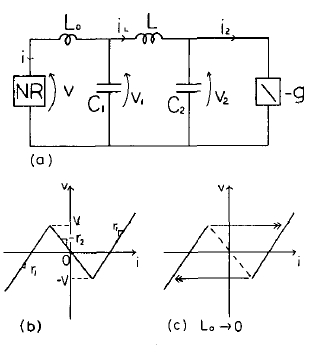
\includegraphics[width=0.5\textwidth]{Saito/fig. 1 Saito.png}
    \caption{Hyperchaos generator.}
    \label{fig1:saito}
\end{figure}
In this circuit, - g is a linear negative conductor characterized by i, = - gv, and NR is a current-controlled nonlinear resistor characterized by a piecewise-linear function of Fig. \ref{fig1:saito}(b):

\begin{equation}
    v= f(i) =
        \left\{
        	\begin{array}{ll}
        		r_{1}(i-1)-V & \mbox{if } i > I \\ %\geq
        		-r_{2}i & \mbox{if } |i| < I; I \equiv V/r_{2}\\
                r_{1}(i+1)+V & \mbox{if } i < I 
        	\end{array}
        \right.
\end{equation}

Some experimental facts show that NR operates as a hysteresis resistor of Fig. \ref{fig1:saito}(c) if the small inductor $L_0$ is shorted. NR and - g are easily realized by circuitries in Fig. \ref{fig2:saito}. In order to simplify the arguments, it is assumed that the op amp is linear and that the zener diode is ideal. The circuit dynamics are described by the basic equation:

\begin{equation}
        \left\{
        	\begin{array}{ll} 
           \vspace{2mm}
           C_{1}\dfrac{dv_{1}}{dt}=-i_{L}-i\\
           \vspace{2mm}
           C_{2}\dfrac{dv_{2}}{dt}=gv_{2}+i_{2}\\
           \vspace{2mm}
           L\dfrac{di_{L}}{dt}=v_{1}-v_{2}\\
           \vspace{2mm}
           L_{0}\dfrac{di}{dt}=v_{1}-f(i), & L_{0}:small.
        	\end{array}
        \right.
\end{equation}

Notice at first, (2) is transformed into a canonical form equation which includes one small parameter $\epsilon$ ($\propto L_0$).
Letting $\epsilon$ tend to zero, the equation is simplified into a constrained system, and a two-dimensional Poincare map can be rigorously derived from it. Laboratory experiments indicate bifurcations from periodic to quasi-periodic solutions (so-called torus) and then to different types of chaotic solutions. These data are reproduced by numerical solutions of the constrained system. The Poincare map and its Lyapunov exponents verify the generation of hyperchaos and related phenomena.

\begin{figure}[h!]
    \centering
    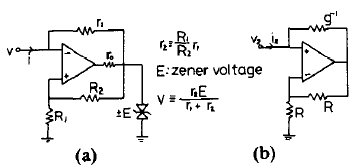
\includegraphics[width=0.4\textwidth]{Saito/fig. 2 saito.png}
    \caption{Realization of NR and -g.}
    \label{fig2:saito}
\end{figure}
\vspace{5mm}
\textbf{EXPERIMENTS}\\
The circuit of Fig. 1 exhibits various interesting phenomena. Some laboratory measurements and their numerical confirmations are shown in this section. Also, we note that the condition (10) is satisfied for these results.

\begin{figure}[h]
    \centering
    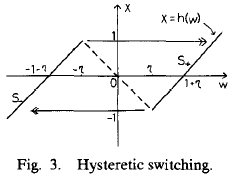
\includegraphics[width=0.3\textwidth]{Saito/fig. 3 Saito.png}
    \caption{fig. 3 Saito}
    \label{fig.3:saito}
\end{figure}

\begin{figure}[h]
    \centering
    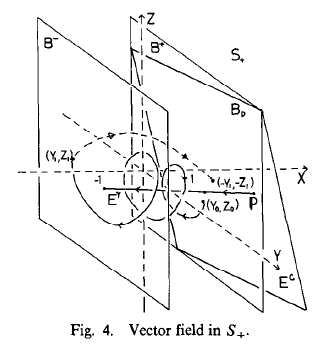
\includegraphics[width=0.3\textwidth]{Saito/fig. 4 Saito.png}
    \caption{fig. 4 Saito}
    \label{fig.4:saito}
\end{figure}

\begin{figure}[h]
    \centering
    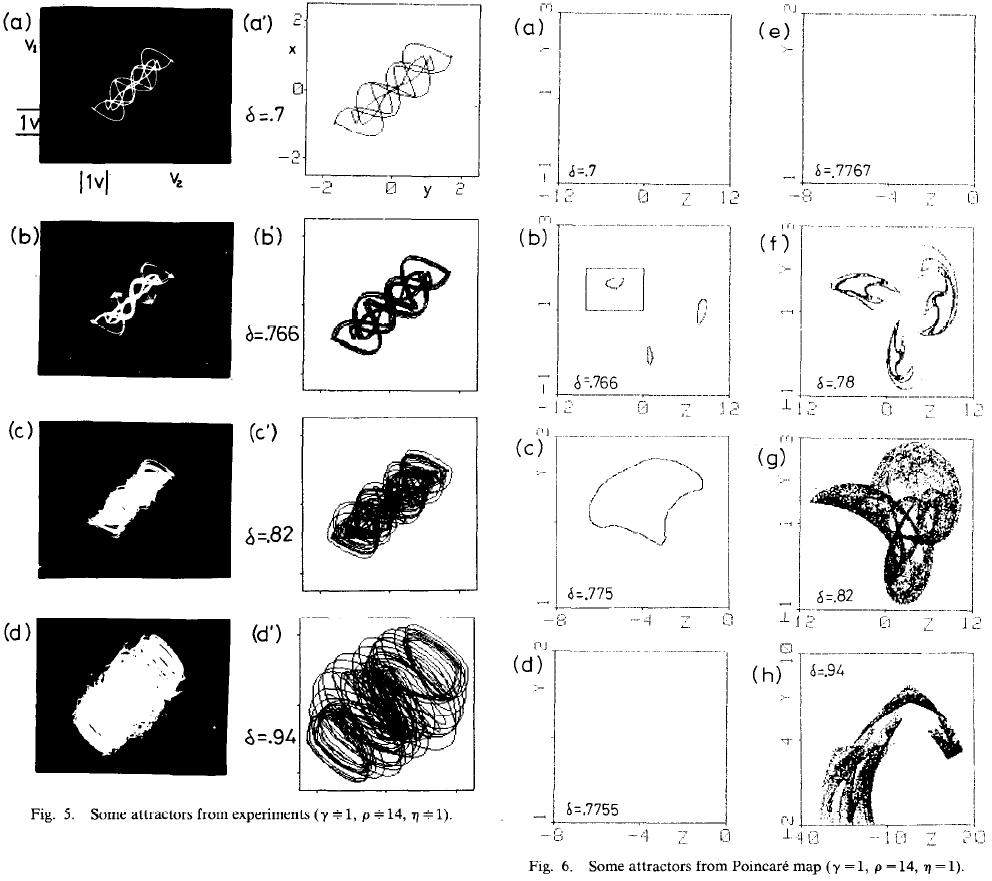
\includegraphics[width=0.3\textwidth]{Saito/fig. 5 6 Saito.png}
    \caption{...}
    \label{fig.5-6:saito}
\end{figure}

\begin{figure}[h]
    \centering
    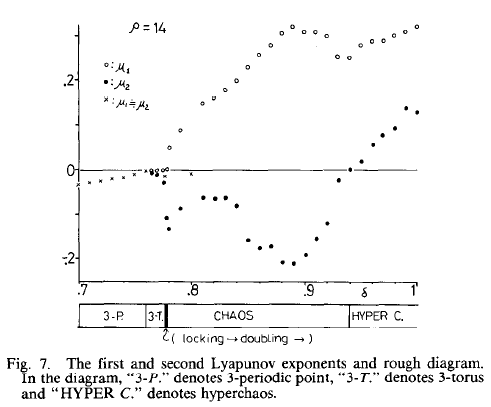
\includegraphics[width=0.3\textwidth]{Saito/fig 7 Saito.png}
    \caption{fig. 7 Saito}
    \label{fig.7:saito}
\end{figure}
%\clearpage

%%%%%%%%%%%%%%%%%%%%%%%%%%%%%%%%%%%%%%%%%%%%%%%%%%%%%%%%%%%%%%%%%%%

\section{RL Diode circuit}
El circuito RLD (Fig. \ref{fig1:RL Diode}) se comportará alternativamente en dos modos diferentes cuando esté sometido a una fuente de tensión alterna: el primero cuando el diodo esté polarizado hacia delante y el otro cuando esté polarizado hacia atrás.

\begin{figure}[h]
    \centering
    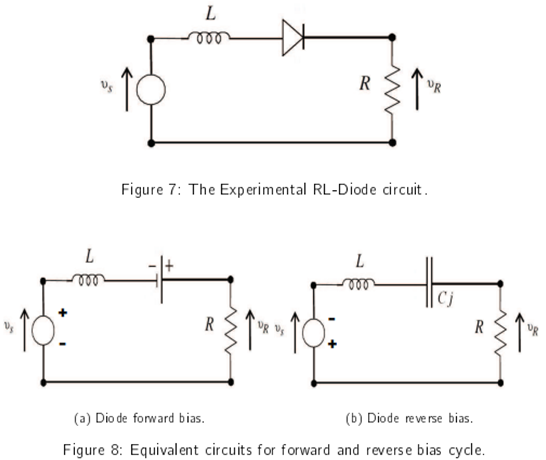
\includegraphics[width=0.5\textwidth]{RLDiodo/fig 1 rldiode.png}
    \caption{RL Diode.}
    \label{fig1:RL Diode}
\end{figure}

Durante el ciclo de conducción, el circuito se reduce a lo que se muestra en la Fig. \ref{fig1:RL Diode} (a), con el diodo actuando como una caída de tensión fija, es decir, como una pila. La ley de tensión de Kirchoffs aplicada a este circuito da:
\begin{equation}
    LdI/dt + RI = V_{0}sin(wt) + V_f
\end{equation}
donde $V_o$ es la amplitud de pico de la tensión alterna de entrada y $V_f$ es la caída de tensión directa del diodo, que suele ser de unos 0.5-1.0 V. La solución de esta ecuación, es decir, la corriente en el ciclo de conducción se encuentra fácilmente [4]:
\begin{equation}
    I(t) = (V_{0}/Z_a)cos(wt-\omega) + V_{f}/R + A\exp{-Rt/L}
\end{equation}
En la ecuación anterior $\theta = tan^(-1)⁡(-ωL/R)$ representa un retardo de fase; A es una constante de integración que se calcula utilizando las condiciones iníciales y $Z_{a}=\sqrt{R^{2}+ω^{2}L^{2}}$ es la impedancia de polarización directa del circuito.
En el ciclo no conductor, el diodo se comporta como un condensador con una capacitancia igual a su capacitancia de unión ($C_j$). El circuito equivalente puede representarse como un circuito RLC conducido (Fig. \ref{fig1:RL Diode}(b)). La ecuación de bucle se convierte en una ecuación diferencial de segundo orden:
\begin{equation}
    Ld^{2}I/dt{^2} + RdI/dt + (1/C_{j})I = V_{0}wcos(wt)
\end{equation}
cuya solución es:
\begin{equation}
    I(t) = (V_{0}/Z_b)cos(wt-\omega_b) + B\exp{-Rt/2L}cos(w_{b}t-\theta)
\end{equation}
Las constantes B y $\phi$ son constantes de integración y pueden hallarse utilizando las condiciones iniciales del ciclo. Además, $\theta_b = tan^(-1)⁡(ωR/L(w_{0}^{2}-w^{2})$, $w_{0}^{2}=(1/LC_j)$, $w_{b}^{2} = w_{0}^{2}-(R/2L)^2$ y $Z_{b}=(L/w)\sqrt{(R^{2}+ω^{2}L^{2}){^2}+(Rw/L)^2}$.
El tiempo de recuperación de un diodo es el tiempo que tardaría un diodo en detener completamente el paso de la corriente directa a través de sí mismo cuando pasa al ciclo no conductor. Depende de la cantidad de corriente de avance máxima que acaba de pasar por el diodo. Cuanto mayor sea la corriente de avance máxima, mayor será el tiempo de recuperación del diodo. En términos cuantitativos, el tiempo de recuperación viene dado por [4]:
\begin{equation}
    \tau_r = \tau_{m}(1-\exp{-|I_m|/I_c})
\end{equation}
donde $|I_m|$ es la magnitud de la corriente de avance máxima más reciente, y $|τ_m|$ e $|I_c|$ son parámetros de fabricación para el diodo específico.

\textbf{La ruta del caos por duplicación de periodos}

Una cierta cantidad de corriente inversa fluirá a través del diodo en cada ciclo de polarización inversa debido al tiempo de recuperación finito del diodo. Si la corriente de pico lm es grande en el ciclo de conducción (figura (9), intervalo 'a'), el diodo se apagará con un cierto retardo (figura (9), intervalo 'b'] debido al tiempo de recuperación finito y así permitirá que fluya una corriente incluso en el ciclo de polarización inversa (mostrado en el intervalo 'b'). Esta corriente inversa, a su vez, impedirá que el diodo se encienda instantáneamente en el ciclo de polarización hacia delante: se encenderá con un retardo (figura (9), intervalo 'c']. Esto mantendrá el pico de corriente hacia delante más pequeño que en el ciclo de polarización hacia delante anterior, dando lugar a dos picos distintos de la corriente hacia delante. Observe que en este proceso se necesitaron dos ciclos de la señal de conducción. Esto es lo que identificamos como una bifurcación de duplicación de periodo. Cuando se aumenta el valor pico de la tensión de conducción, puede producirse una bifurcación a período 4 seguida, posiblemente, por bifurcaciones superiores y, finalmente, el caos.
\begin{figure}
    \centering
    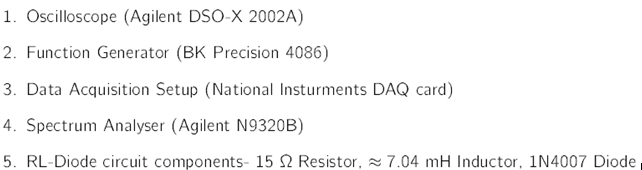
\includegraphics[width=0.4\textwidth]{RLDiodo/fig rldiode materiales.png}
    \caption{RLDiode materiales de laboratorio.}
    \label{fig:RLDiode materiales}
\end{figure}
El circuito RLD la corriente y la tensión se harán oscilar utilizando una señal de corriente alterna. La señal se controla a través de dos parámetros: frecuencia y amplitud. Así que tenemos la opción de mantener uno de ellos constante y cambiar el otro. En nuestro caso la frecuencia se mantendrá constante mientras que la amplitud se varía. (Fix the frequency of VIN using the BK4086 signal generator to 50 kHz.)

%\clearpage

%%%%%%%%%%%%%%%%%%%%%%%%%%%%%%%%%%%%%%%%%%%%%%%%%%%%%%%%%%%%%%%%%%
\section{Chua's circuit}
Entre los sistemas caóticos más típicos y de fácil acceso figuran los circuitos electrónicos. kennedy1993three menciona que deben satisfacerse tres criterios relacionados con los elementos que deben tener los circuitos: 

(i) Al menos un elemento no lineal.

(ii) Al menos una resistencia localmente activa (resistencia negativa). 

(iii) Tres o más elementos de almacenamiento de energía.

El circuito de Chua (Fig.~\ref{fig:circuito de Chua}) cumple estos criterios y es uno de los más populares que exhibe caos, puesto que es un circuito autónomo simple capaz de mostrar comportamiento caótico; está compuesto, por una porción que presenta el comportamiento típico de un oscilador amortiguado (dos condensadores $C_1$ y $C_2$, una resistencia variable $R$ y una bobina $L$) y la otra parte que constituye el único elemento no lineal denominado diodo de Chua, $N_R$ que básicamente es una resistencia no lineal negativa o lineal por partes (piecewise linear o PWL) como se muestra en la Fig.~\ref{fig:diodo teórico}. Este elemento causante de la no linealidad actúa como la fuente de energía de todo el circuito, ya que es la responsable de la retroalimentación que lo mantiene oscilando. 
\begin{figure}[h]
    \centering
    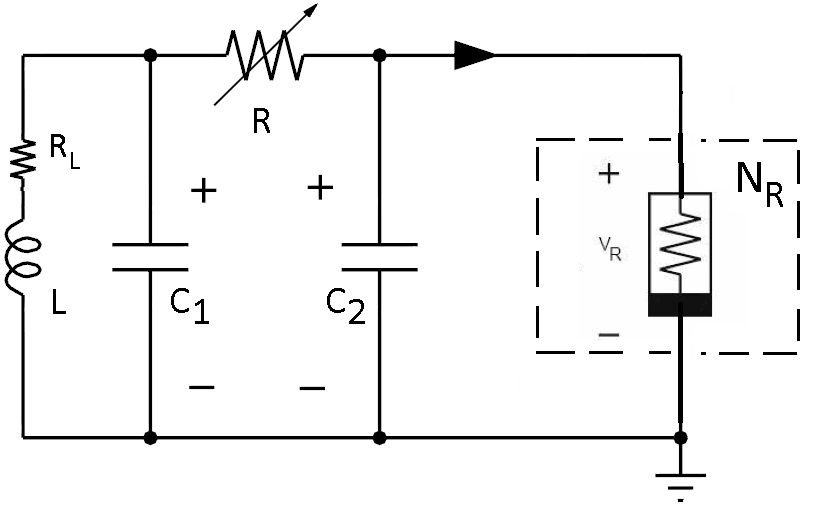
\includegraphics[width=0.45\textwidth]{Chua/circuitodechua.png}
    \caption{\label{fig:circuito de Chua} Circuito de Chua canónico.}
\end{figure}
Escribiendo las variables dinámicas $V_{C_1}$, $V_{C_2}$ e $I_L$, junto con los voltajes de quiebre $-B_{p}$ y $+B_{p}$, como:
%Ec. 1
\begin{eqnarray}
    \begin{aligned}
        x & = V_{C_1}(B_p)^{-1},\\
        y & = V_{C_2}(B_p)^{-1},\\ 
        z & = RI_L(B_p)^{-1},\\ 
        \tau & = t(RC_2)^{-1},
    \end{aligned}
\end{eqnarray}
se obtiene las ecuaciones diferenciales adimen\-sio\-na\-les:
%Ec. 2
\begin{eqnarray}\label{Chua eq dif}
    %\centering
    \begin{aligned}
        %\frac{\text{d}x}{\text{d}\tau} &= \alpha(y - x - f(x)),\\
        %\frac{\text{d}y}{\text{d}\tau} &= x-y+z,\\
        %\frac{\text{d}z}{\text{d}\tau} &= -\beta y - \gamma z,
        \dot{x} &= \alpha(y - x - f(x)),\\
        \dot{y} &= x-y+z,\\
        \dot{z} &= -\beta y - \gamma z,
    \end{aligned}
\end{eqnarray}
con los parámetros:
%Ec. 3
\begin{eqnarray}\label{alfa beta gamma}
    \begin{aligned}
        \alpha & = C_{2} C_{3}^{-1},\\
        \beta & = R^{2} C_2 L^{-1}, \\
        \gamma & = R_{L} RC_{2} L^{-1},
    \end{aligned}
\end{eqnarray}
donde $R_L$ representa la resistencia interna del inductor $L$ en la Fig.~\ref{fig:circuito de Chua}. A esta configuración se la conoce como circuito de Chua canónico ($\mathfrak{C}^2$), en el sentido de que puede exhibir todos los posibles comportamientos dinámicos asociados con cualquier campo vector continuo, lineal por partes (PWL) y simétrico de tres regiones. En el caso de no con\-si\-de\-rar la resistencia $R_L$, el valor de $\gamma$ es nulo y el circuito de Chua ($\mathfrak{C}^1$) se convierte en el caso simple/ideal.
\begin{figure}[h]
    \centering
    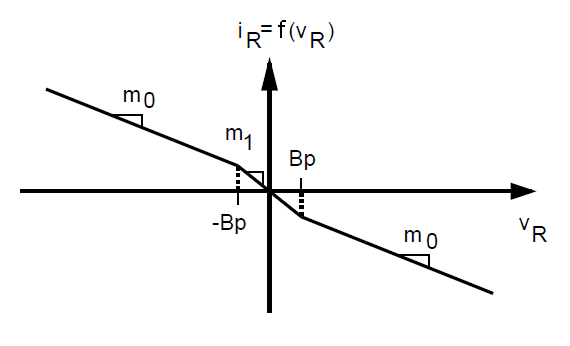
\includegraphics[width=0.4\textwidth]{Chua/DiodoChua.png}
    \caption{Característica de linealidad por partes de voltaje y corriente del diodo de Chua. $-B_{p}$ y $+B_{p}$ son los puntos de quiebre de la relación corriente-voltaje del diodo de Chua; en tanto que $m_{0}$ y $m_{1}$ son las pendientes de la región externa e interna, respectivamente (kennedy1992robust).} 
    \label{fig:diodo teórico}
\end{figure} 
La función PWL que describe el comportamiento del diodo de Chua, es:
%Ec. 4
\begin{equation}\label{f(x) PWL}
    f(x) = m_{0}x + (1/2)(m_{1}-m_{0})(|x+B_p|-|x-B_p|),
\end{equation}
las pendientes $m_0$ y $m_1$ se pueden escribir como:
%Ec. 5
\begin{eqnarray}\label{pendientes}
    \begin{aligned}
        m_0=(-R_3^{-1} +R_4^{-1}),\\
        m_1=(-R_3^{-1} -R_6^{-1}).
    \end{aligned}
\end{eqnarray}

\subsection{Bifurcations in the chua circuit}
\begin{figure*}
    %\centering
    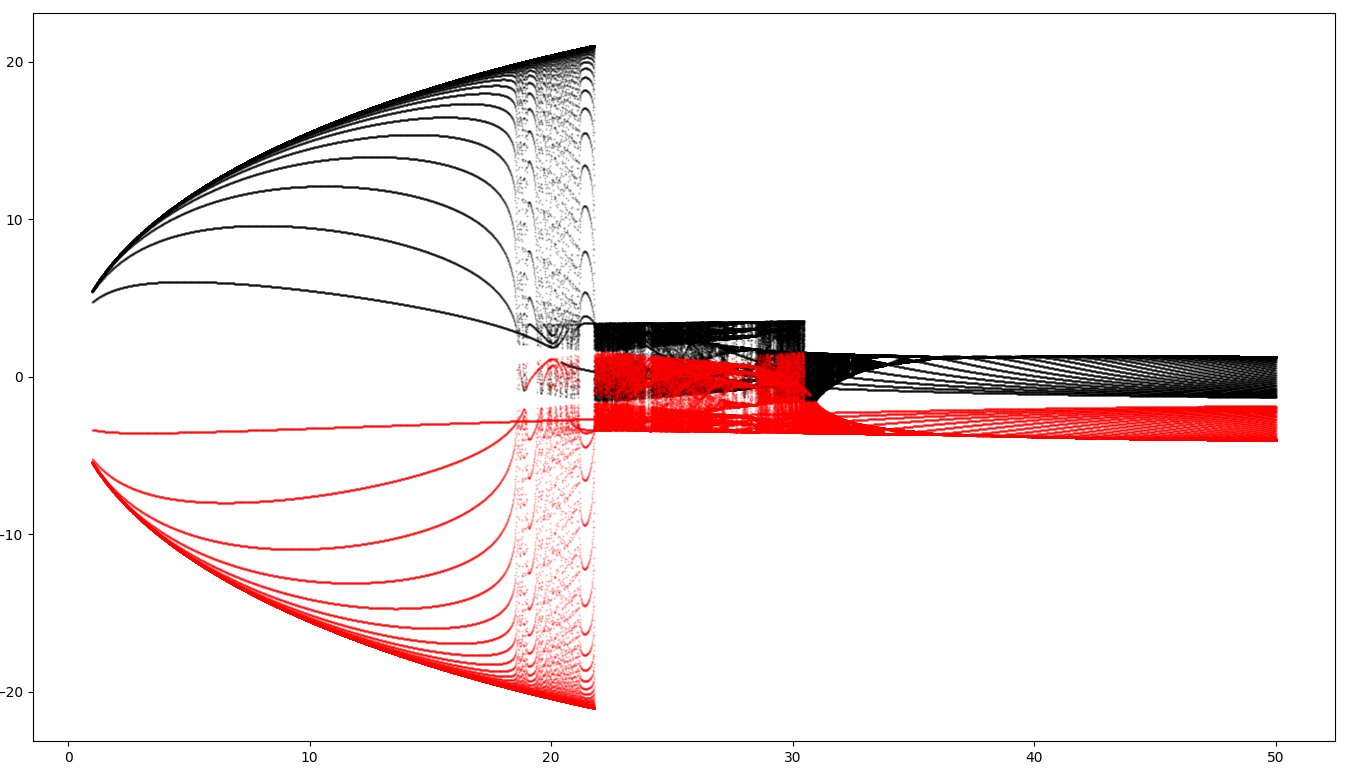
\includegraphics[width=\textwidth]{Chua/0_50s_Chua.png}
    \caption{\label{fig:circuito de Chua} eeeaaBifurcations in the chua circuit with parameter in 0-50s.}
\end{figure*}
%\clearpage
%%%%%%%%%%%%%%%%%%%%%%%%%%%%%%%%%%%%%%%%%%%%%%%%%%%
\section{Lorenz System}
The Lorenz system is a system of ordinary differential equations first studied by mathematician and meteorologist Edward Lorenz. It is notable for having chaotic solutions for certain parameter values and initial conditions. In particular, the Lorenz attractor is a set of chaotic solutions of the Lorenz system. This underscores that physical systems can be completely deterministic and yet still be inherently unpredictable. 
In 1963, Edward Lorenz, with the help of Ellen Fetter who was responsible for the numerical simulations and figures, and Margaret Hamilton who helped in the initial, numerical computations leading up to the findings of the Lorenz model, developed a simplified mathematical model for atmospheric convection. The model is a system of three ordinary differential equations now known as the Lorenz equations:
\begin{eqnarray}\label{Chua eq dif}
    %\centering
    \begin{aligned}
        \dot{x} &= \sigma(y - x),\\
        \dot{y} &= x(\rho - z),\\
        \dot{z} &= x y - \beta z.
    \end{aligned}
\end{eqnarray}

\begin{figure*}
    \centering
    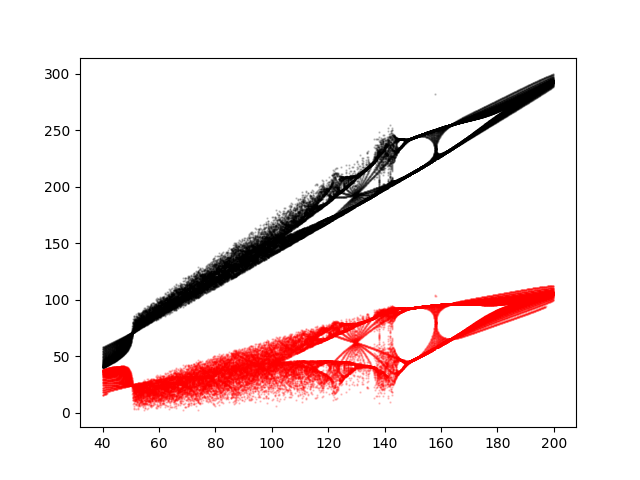
\includegraphics[\textwidth]{Lorenz/Lorenz_Bif_mismo_u0_1.png}
    \caption{\label{fig:Lorenz Bifurcation} Bifurcation of the Lorenz system with "fixed" initial condition.}
\end{figure*}

\begin{figure*}
    \centering
    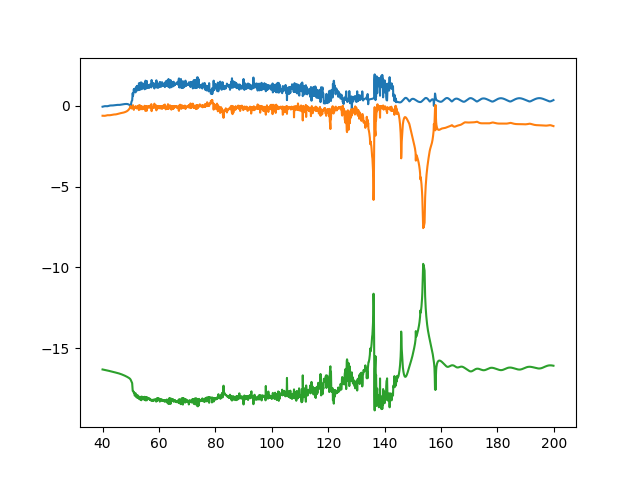
\includegraphics[\textwidth]{Lorenz/Lorenz_Lyap_exp.png}
    \caption{\label{Lorenz exponent Lyapunov} Lyapinov exponent of the Lorenz system with "fixed" initial condition.}
\end{figure*}

%\clearpage
%%%%%%%%%%%%%%%%%%%%%%%%%%%%%%%%%%%%%%%%%%%%%%%%
\section{Henon map}
The Henon map, dynamical system two-dimensional, defined as:
\begin{equation}
    \begin{aligned}
        x_{n+1} = 1 - a x_{n}^{2} + y_{n},\\
        y_{n+1} = b x_{n},
    \end{aligned}
\end{equation}
with parameters $a=1.4,b=0.3$ and the inicial condition $x_0 = 0.2, y_0 = 0.3$. For a time of $n=10 000$ we obtain Fig. \ref{Henon_fig_1} of its trajectory (which actually has 10 001 data for the zero included).
\begin{figure}[h!]
    \centering
    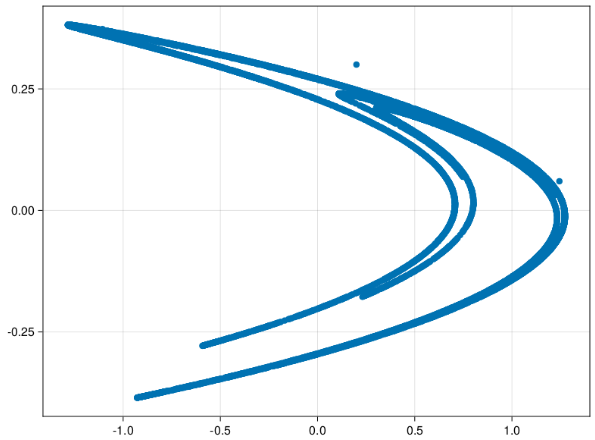
\includegraphics[width=0.4\textwidth]{Henon/Screenshot_1.png}
    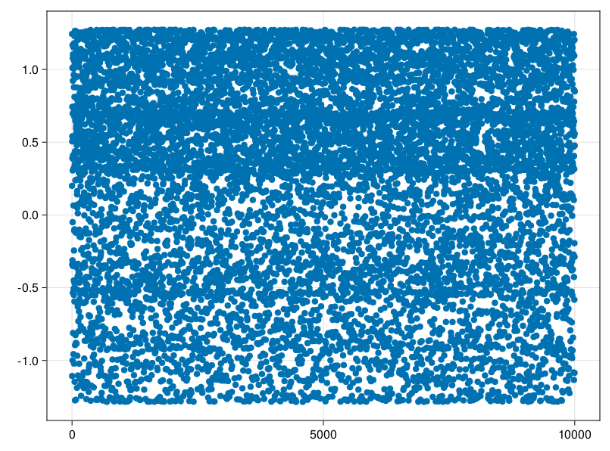
\includegraphics[width=0.5\textwidth]{Henon/Screenshot_2.png}
    \caption{Caption}
    \label{Henon_fig_1}
\end{figure}
%\clearpage

%%%%%%%%%%%%%%%%%%%%%%%%%%%%%%%%%%%%%%%%%5
\section{\label{sec:level1}First-level heading:\protect\\ The line
break was forced \lowercase{via} \textbackslash\textbackslash}

This sample document demonstrates proper use of REV\TeX~4.2 (and
\LaTeXe) in mansucripts prepared for submission to APS
journals. Further information can be found in the REV\TeX~4.2
documentation included in the distribution or available at
\url{http://journals.aps.org/revtex/}.

When commands are referred to in this example file, they are always
shown with their required arguments, using normal \TeX{} format. In
this format, \verb+#1+, \verb+#2+, etc. stand for required
author-supplied arguments to commands. For example, in
\verb+\section{#1}+ the \verb+#1+ stands for the title text of the
author's section heading, and in \verb+\title{#1}+ the \verb+#1+
stands for the title text of the paper.

Line breaks in section headings at all levels can be introduced using
\textbackslash\textbackslash. A blank input line tells \TeX\ that the
paragraph has ended. Note that top-level section headings are
automatically uppercased. If a specific letter or word should appear in
lowercase instead, you must escape it using \verb+\lowercase{#1}+ as
in the word ``via'' above.

\subsection{\label{sec:level2}Second-level heading: Formatting}

This file may be formatted in either the \texttt{preprint} or
\texttt{reprint} style. \texttt{reprint} format mimics final journal output. 
Either format may be used for submission purposes. \texttt{letter} sized paper should
be used when submitting to APS journals.

\subsubsection{Wide text (A level-3 head)}
The \texttt{widetext} environment will make the text the width of the
full page, as on page~\pageref{eq:wideeq}. (Note the use the
\verb+\pageref{#1}+ command to refer to the page number.) 
\paragraph{Note (Fourth-level head is run in)}
The width-changing commands only take effect in two-column formatting. 
There is no effect if text is in a single column.

\subsection{\label{sec:citeref}Citations and References}
A citation in text uses the command \verb+\cite{#1}+ or
\verb+\onlinecite{#1}+ and refers to an entry in the bibliography. 
An entry in the bibliography is a reference to another document.

\subsubsection{Citations}
Because REV\TeX\ uses the \verb+natbib+ package of Patrick Daly, 
the entire repertoire of commands in that package are available for your document;
see the \verb+natbib+ documentation for further details. Please note that
REV\TeX\ requires version 8.31a or later of \verb+natbib+.

\paragraph{Syntax}
The argument of \verb+\cite+ may be a single \emph{key}, 
or may consist of a comma-separated list of keys.
The citation \emph{key} may contain 
letters, numbers, the dash (-) character, or the period (.) character. 
New with natbib 8.3 is an extension to the syntax that allows for 
a star (*) form and two optional arguments on the citation key itself.
The syntax of the \verb+\cite+ command is thus (informally stated)
\begin{quotation}\flushleft\leftskip1em
\verb+\cite+ \verb+{+ \emph{key} \verb+}+, or\\
\verb+\cite+ \verb+{+ \emph{optarg+key} \verb+}+, or\\
\verb+\cite+ \verb+{+ \emph{optarg+key} \verb+,+ \emph{optarg+key}\ldots \verb+}+,
\end{quotation}\noindent
where \emph{optarg+key} signifies 
\begin{quotation}\flushleft\leftskip1em
\emph{key}, or\\
\texttt{*}\emph{key}, or\\
\texttt{[}\emph{pre}\texttt{]}\emph{key}, or\\
\texttt{[}\emph{pre}\texttt{]}\texttt{[}\emph{post}\texttt{]}\emph{key}, or even\\
\texttt{*}\texttt{[}\emph{pre}\texttt{]}\texttt{[}\emph{post}\texttt{]}\emph{key}.
\end{quotation}\noindent
where \emph{pre} and \emph{post} is whatever text you wish to place 
at the beginning and end, respectively, of the bibliographic reference
(see Ref.~[\onlinecite{witten2001}] and the two under Ref.~[\onlinecite{feyn54}]).
(Keep in mind that no automatic space or punctuation is applied.)
It is highly recommended that you put the entire \emph{pre} or \emph{post} portion 
within its own set of braces, for example: 
\verb+\cite+ \verb+{+ \texttt{[} \verb+{+\emph{text}\verb+}+\texttt{]}\emph{key}\verb+}+.
The extra set of braces will keep \LaTeX\ out of trouble if your \emph{text} contains the comma (,) character.

The star (*) modifier to the \emph{key} signifies that the reference is to be 
merged with the previous reference into a single bibliographic entry, 
a common idiom in APS and AIP articles (see below, Ref.~[\onlinecite{epr}]). 
When references are merged in this way, they are separated by a semicolon instead of 
the period (full stop) that would otherwise appear.

\paragraph{Eliding repeated information}
When a reference is merged, some of its fields may be elided: for example, 
when the author matches that of the previous reference, it is omitted. 
If both author and journal match, both are omitted.
If the journal matches, but the author does not, the journal is replaced by \emph{ibid.},
as exemplified by Ref.~[\onlinecite{epr}]. 
These rules embody common editorial practice in APS and AIP journals and will only
be in effect if the markup features of the APS and AIP Bib\TeX\ styles is employed.

\paragraph{The options of the cite command itself}
Please note that optional arguments to the \emph{key} change the reference in the bibliography, 
not the citation in the body of the document. 
For the latter, use the optional arguments of the \verb+\cite+ command itself:
\verb+\cite+ \texttt{*}\allowbreak
\texttt{[}\emph{pre-cite}\texttt{]}\allowbreak
\texttt{[}\emph{post-cite}\texttt{]}\allowbreak
\verb+{+\emph{key-list}\verb+}+.

\subsubsection{Example citations}
By default, citations are numerical\cite{Beutler1994}.
Author-year citations are used when the journal is RMP. 
To give a textual citation, use \verb+\onlinecite{#1}+: 
Refs.~\onlinecite{[][{, and references therein}]witten2001,Bire82}. 
By default, the \texttt{natbib} package automatically sorts your citations into numerical order and ``compresses'' runs of three or more consecutive numerical citations.
REV\TeX\ provides the ability to automatically change the punctuation when switching between journal styles that provide citations in square brackets and those that use a superscript style instead. This is done through the \texttt{citeautoscript} option. For instance, the journal style \texttt{prb} automatically invokes this option because \textit{Physical 
Review B} uses superscript-style citations. The effect is to move the punctuation, which normally comes after a citation in square brackets, to its proper position before the superscript. 
To illustrate, we cite several together 
\cite{[See the explanation of time travel in ]feyn54,*[The classical relativistic treatment of ][ is a relative classic]epr,witten2001,Berman1983,Davies1998,Bire82}, 
and once again in different order (Refs.~\cite{epr,feyn54,Bire82,Berman1983,witten2001,Davies1998}). 
Note that the citations were both compressed and sorted. Futhermore, running this sample file under the \texttt{prb} option will move the punctuation to the correct place.

When the \verb+prb+ class option is used, the \verb+\cite{#1}+ command
displays the reference's number as a superscript rather than in
square brackets. Note that the location of the \verb+\cite{#1}+
command should be adjusted for the reference style: the superscript
references in \verb+prb+ style must appear after punctuation;
otherwise the reference must appear before any punctuation. This
sample was written for the regular (non-\texttt{prb}) citation style.
The command \verb+\onlinecite{#1}+ in the \texttt{prb} style also
displays the reference on the baseline.

\subsubsection{References}
A reference in the bibliography is specified by a \verb+\bibitem{#1}+ command
with the same argument as the \verb+\cite{#1}+ command.
\verb+\bibitem{#1}+ commands may be crafted by hand or, preferably,
generated by Bib\TeX. 
REV\TeX~4.2 includes Bib\TeX\ style files
\verb+apsrev4-2.bst+, \verb+apsrmp4-2.bst+ appropriate for
\textit{Physical Review} and \textit{Reviews of Modern Physics},
respectively.

\subsubsection{Example references}
This sample file employs the \verb+\bibliography+ command, 
which formats the \texttt{\jobname .bbl} file
and specifies which bibliographic databases are to be used by Bib\TeX\ 
(one of these should be by arXiv convention \texttt{\jobname .bib}).
Running Bib\TeX\ (via \texttt{bibtex \jobname}) 
after the first pass of \LaTeX\ produces the file
\texttt{\jobname .bbl} which contains the automatically formatted
\verb+\bibitem+ commands (including extra markup information via
\verb+\bibinfo+ and \verb+\bibfield+ commands). 
If not using Bib\TeX, you will have to create the \verb+thebibiliography+ environment 
and its \verb+\bibitem+ commands by hand.

Numerous examples of the use of the APS bibliographic entry types appear in the bibliography of this sample document.
You can refer to the \texttt{\jobname .bib} file, 
and compare its information to the formatted bibliography itself.

\subsection{Footnotes}%
Footnotes, produced using the \verb+\footnote{#1}+ command, 
usually integrated into the bibliography alongside the other entries.
Numerical citation styles do this%
\footnote{Automatically placing footnotes into the bibliography requires using BibTeX to compile the bibliography.};
author-year citation styles place the footnote at the bottom of the text column.
Note: due to the method used to place footnotes in the bibliography, 
\emph{you must re-run Bib\TeX\ every time you change any of your document's footnotes}. 

\section{Math and Equations}
Inline math may be typeset using the \verb+$+ delimiters. Bold math
symbols may be achieved using the \verb+bm+ package and the
\verb+\bm{#1}+ command it supplies. For instance, a bold $\alpha$ can
be typeset as \verb+$\bm{\alpha}$+ giving $\bm{\alpha}$. Fraktur and
Blackboard (or open face or double struck) characters should be
typeset using the \verb+\mathfrak{#1}+ and \verb+\mathbb{#1}+ commands
respectively. Both are supplied by the \texttt{amssymb} package. For
example, \verb+$\mathbb{R}$+ gives $\mathbb{R}$ and
\verb+$\mathfrak{G}$+ gives $\mathfrak{G}$

In \LaTeX\ there are many different ways to display equations, and a
few preferred ways are noted below. Displayed math will center by
default. Use the class option \verb+fleqn+ to flush equations left.

Below we have numbered single-line equations; this is the most common
type of equation in \textit{Physical Review}:
\begin{eqnarray}
\chi_+(p)\alt{\bf [}2|{\bf p}|(|{\bf p}|+p_z){\bf ]}^{-1/2}
\left(
\begin{array}{c}
|{\bf p}|+p_z\\
px+ip_y
\end{array}\right)\;,
\\
\left\{%
 \openone234567890abc123\alpha\beta\gamma\delta1234556\alpha\beta
 \frac{1\sum^{a}_{b}}{A^2}%
\right\}%
\label{eq:one}.
\end{eqnarray}
Note the open one in Eq.~(\ref{eq:one}).

Not all numbered equations will fit within a narrow column this
way. The equation number will move down automatically if it cannot fit
on the same line with a one-line equation:
\begin{equation}
\left\{
 ab12345678abc123456abcdef\alpha\beta\gamma\delta1234556\alpha\beta
 \frac{1\sum^{a}_{b}}{A^2}%
\right\}.
\end{equation}

When the \verb+\label{#1}+ command is used [cf. input for
Eq.~(\ref{eq:one})], the equation can be referred to in text without
knowing the equation number that \TeX\ will assign to it. Just
use \verb+\ref{#1}+, where \verb+#1+ is the same name that used in
the \verb+\label{#1}+ command.

Unnumbered single-line equations can be typeset
using the \verb+\[+, \verb+\]+ format:
\[g^+g^+ \rightarrow g^+g^+g^+g^+ \dots ~,~~q^+q^+\rightarrow
q^+g^+g^+ \dots ~. \]


\subsection{Multiline equations}

Multiline equations are obtained by using the \verb+eqnarray+
environment.  Use the \verb+\nonumber+ command at the end of each line
to avoid assigning a number:
\begin{eqnarray}
{\cal M}=&&ig_Z^2(4E_1E_2)^{1/2}(l_i^2)^{-1}
\delta_{\sigma_1,-\sigma_2}
(g_{\sigma_2}^e)^2\chi_{-\sigma_2}(p_2)\nonumber\\
&&\times
[\epsilon_jl_i\epsilon_i]_{\sigma_1}\chi_{\sigma_1}(p_1),
\end{eqnarray}
\begin{eqnarray}
\sum \vert M^{\text{viol}}_g \vert ^2&=&g^{2n-4}_S(Q^2)~N^{n-2}
        (N^2-1)\nonumber \\
 & &\times \left( \sum_{i<j}\right)
  \sum_{\text{perm}}
 \frac{1}{S_{12}}
 \frac{1}{S_{12}}
 \sum_\tau c^f_\tau~.
\end{eqnarray}
\textbf{Note:} Do not use \verb+\label{#1}+ on a line of a multiline
equation if \verb+\nonumber+ is also used on that line. Incorrect
cross-referencing will result. Notice the use \verb+\text{#1}+ for
using a Roman font within a math environment.

To set a multiline equation without \emph{any} equation
numbers, use the \verb+\begin{eqnarray*}+,
\verb+\end{eqnarray*}+ format:
\begin{eqnarray*}
\sum \vert M^{\text{viol}}_g \vert ^2&=&g^{2n-4}_S(Q^2)~N^{n-2}
        (N^2-1)\\
 & &\times \left( \sum_{i<j}\right)
 \left(
  \sum_{\text{perm}}\frac{1}{S_{12}S_{23}S_{n1}}
 \right)
 \frac{1}{S_{12}}~.
\end{eqnarray*}

To obtain numbers not normally produced by the automatic numbering,
use the \verb+\tag{#1}+ command, where \verb+#1+ is the desired
equation number. For example, to get an equation number of
(\ref{eq:mynum}),
\begin{equation}
g^+g^+ \rightarrow g^+g^+g^+g^+ \dots ~,~~q^+q^+\rightarrow
q^+g^+g^+ \dots ~. \tag{2.6$'$}\label{eq:mynum}
\end{equation}

\paragraph{A few notes on \texttt{tag}s} 
\verb+\tag{#1}+ requires the \texttt{amsmath} package. 
Place the \verb+\tag{#1}+ command before the \verb+\label{#1}+, if any. 
The numbering produced by \verb+\tag{#1}+ \textit{does not affect} 
the automatic numbering in REV\TeX; 
therefore, the number must be known ahead of time, 
and it must be manually adjusted if other equations are added. 
\verb+\tag{#1}+ works with both single-line and multiline equations. 
\verb+\tag{#1}+ should only be used in exceptional cases---%
do not use it to number many equations in your paper. 
Please note that this feature of the \texttt{amsmath} package
is \emph{not} compatible with the \texttt{hyperref} (6.77u) package.

Enclosing display math within
\verb+\begin{subequations}+ and \verb+\end{subequations}+ will produce
a set of equations that are labeled with letters, as shown in
Eqs.~(\ref{subeq:1}) and (\ref{subeq:2}) below.
You may include any number of single-line and multiline equations,
although it is probably not a good idea to follow one display math
directly after another.
\begin{subequations}
\label{eq:whole}
\begin{eqnarray}
{\cal M}=&&ig_Z^2(4E_1E_2)^{1/2}(l_i^2)^{-1}
(g_{\sigma_2}^e)^2\chi_{-\sigma_2}(p_2)\nonumber\\
&&\times
[\epsilon_i]_{\sigma_1}\chi_{\sigma_1}(p_1).\label{subeq:2}
\end{eqnarray}
\begin{equation}
\left\{
 abc123456abcdef\alpha\beta\gamma\delta1234556\alpha\beta
 \frac{1\sum^{a}_{b}}{A^2}
\right\},\label{subeq:1}
\end{equation}
\end{subequations}
Giving a \verb+\label{#1}+ command directly after the \verb+\begin{subequations}+, 
allows you to reference all the equations in the \texttt{subequations} environment. 
For example, the equations in the preceding subequations environment were
Eqs.~(\ref{eq:whole}).

\subsubsection{Wide equations}
The equation that follows is set in a wide format, i.e., it spans the full page. 
The wide format is reserved for long equations
that cannot easily be set in a single column:
\begin{widetext}
\begin{equation}
{\cal R}^{(\text{d})}=
 g_{\sigma_2}^e
 \left(
   \frac{[\Gamma^Z(3,21)]_{\sigma_1}}{Q_{12}^2-M_W^2}
  +\frac{[\Gamma^Z(13,2)]_{\sigma_1}}{Q_{13}^2-M_W^2}
 \right)
 + x_WQ_e
 \left(
   \frac{[\Gamma^\gamma(3,21)]_{\sigma_1}}{Q_{12}^2-M_W^2}
  +\frac{[\Gamma^\gamma(13,2)]_{\sigma_1}}{Q_{13}^2-M_W^2}
 \right)\;. 
 \label{eq:wideeq}
\end{equation}
\end{widetext}
This is typed to show how the output appears in wide format.
(Incidentally, since there is no blank line between the \texttt{equation} environment above 
and the start of this paragraph, this paragraph is not indented.)

\section{Cross-referencing}
REV\TeX{} will automatically number such things as
sections, footnotes, equations, figure captions, and table captions. 
In order to reference them in text, use the
\verb+\label{#1}+ and \verb+\ref{#1}+ commands. 
To reference a particular page, use the \verb+\pageref{#1}+ command.

The \verb+\label{#1}+ should appear 
within the section heading, 
within the footnote text, 
within the equation, or 
within the table or figure caption. 
The \verb+\ref{#1}+ command
is used in text at the point where the reference is to be displayed.  
Some examples: Section~\ref{sec:level1} on page~\pageref{sec:level1},
Table~\ref{tab:table1},%
\begin{table}[b]%The best place to locate the table environment is directly after its first reference in text
\caption{\label{tab:table1}%
A table that fits into a single column of a two-column layout. 
Note that REV\TeX~4 adjusts the intercolumn spacing so that the table fills the
entire width of the column. Table captions are numbered
automatically. 
This table illustrates left-, center-, decimal- and right-aligned columns,
along with the use of the \texttt{ruledtabular} environment which sets the 
Scotch (double) rules above and below the alignment, per APS style.
}
\begin{ruledtabular}
\begin{tabular}{lcdr}
\textrm{Left\footnote{Note a.}}&
\textrm{Centered\footnote{Note b.}}&
\multicolumn{1}{c}{\textrm{Decimal}}&
\textrm{Right}\\
\colrule
1 & 2 & 3.001 & 4\\
10 & 20 & 30 & 40\\
100 & 200 & 300.0 & 400\\
\end{tabular}
\end{ruledtabular}
\end{table}
and Fig.~\ref{fig:epsart}.%
\begin{figure}[b]
\includegraphics{fig_1}% Here is how to import EPS art
\caption{\label{fig:epsart} A figure caption. The figure captions are
automatically numbered.}
\end{figure}

\section{Floats: Figures, Tables, Videos, etc.}
Figures and tables are usually allowed to ``float'', which means that their
placement is determined by \LaTeX, while the document is being typeset. 

Use the \texttt{figure} environment for a figure, the \texttt{table} environment for a table.
In each case, use the \verb+\caption+ command within to give the text of the
figure or table caption along with the \verb+\label+ command to provide
a key for referring to this figure or table.
The typical content of a figure is an image of some kind; 
that of a table is an alignment.%
\begin{figure}
\includegraphics{fig_2}% Here is how to import EPS art
\caption{\label{fig:wide}Use the figure environment to get a wide
figure that spans the page in \texttt{twocolumn} formatting.}
\end{figure}

\begin{table*}
\caption{\label{tab:table3}This is a wide table that spans the full page
width in a two-column layout. It is formatted using the
\texttt{table*} environment. It also demonstates the use of
\textbackslash\texttt{multicolumn} in rows with entries that span
more than one column.}
\begin{ruledtabular}
\begin{tabular}{ccccc}
 &\multicolumn{2}{c}{$D_{4h}^1$}&\multicolumn{2}{c}{$D_{4h}^5$}\\
 Ion&1st alternative&2nd alternative&lst alternative
&2nd alternative\\ \hline
 K&$(2e)+(2f)$&$(4i)$ &$(2c)+(2d)$&$(4f)$ \\
 Mn&$(2g)$\footnote{The $z$ parameter of these positions is $z\sim\frac{1}{4}$.}
 &$(a)+(b)+(c)+(d)$&$(4e)$&$(2a)+(2b)$\\
 Cl&$(a)+(b)+(c)+(d)$&$(2g)$\footnotemark[1]
 &$(4e)^{\text{a}}$\\
 He&$(8r)^{\text{a}}$&$(4j)^{\text{a}}$&$(4g)^{\text{a}}$\\
 Ag& &$(4k)^{\text{a}}$& &$(4h)^{\text{a}}$\\
\end{tabular}
\end{ruledtabular}
\end{table*}

Insert an image using either the \texttt{graphics} or
\texttt{graphix} packages, which define the \verb+\includegraphics{#1}+ command.
(The two packages differ in respect of the optional arguments 
used to specify the orientation, scaling, and translation of the image.) 
To create an alignment, use the \texttt{tabular} environment. 

The best place to locate the \texttt{figure} or \texttt{table} environment
is immediately following its first reference in text; this sample document
illustrates this practice for Fig.~\ref{fig:epsart}, which
shows a figure that is small enough to fit in a single column. 

In exceptional cases, you will need to move the float earlier in the document, as was done
with Table~\ref{tab:table3}: \LaTeX's float placement algorithms need to know
about a full-page-width float earlier. 

Fig.~\ref{fig:wide}
has content that is too wide for a single column,
so the \texttt{figure} environment has been used.%
\begin{table}[b]
\caption{\label{tab:table4}%
Numbers in columns Three--Five are aligned with the ``d'' column specifier 
(requires the \texttt{dcolumn} package). 
Non-numeric entries (those entries without a ``.'') in a ``d'' column are aligned on the decimal point. 
Use the ``D'' specifier for more complex layouts. }
\begin{ruledtabular}
\begin{tabular}{ccddd}
One&Two&
\multicolumn{1}{c}{\textrm{Three}}&
\multicolumn{1}{c}{\textrm{Four}}&
\multicolumn{1}{c}{\textrm{Five}}\\
%\mbox{Three}&\mbox{Four}&\mbox{Five}\\
\hline
one&two&\mbox{three}&\mbox{four}&\mbox{five}\\
He&2& 2.77234 & 45672. & 0.69 \\
C\footnote{Some tables require footnotes.}
  &C\footnote{Some tables need more than one footnote.}
  & 12537.64 & 37.66345 & 86.37 \\
\end{tabular}
\end{ruledtabular}
\end{table}

The content of a table is typically a \texttt{tabular} environment, 
giving rows of type in aligned columns. 
Column entries separated by \verb+&+'s, and 
each row ends with \textbackslash\textbackslash. 
The required argument for the \texttt{tabular} environment
specifies how data are aligned in the columns. 
For instance, entries may be centered, left-justified, right-justified, aligned on a decimal
point. 
Extra column-spacing may be be specified as well, 
although REV\TeX~4 sets this spacing so that the columns fill the width of the
table. Horizontal rules are typeset using the \verb+\hline+
command. The doubled (or Scotch) rules that appear at the top and
bottom of a table can be achieved enclosing the \texttt{tabular}
environment within a \texttt{ruledtabular} environment. Rows whose
columns span multiple columns can be typeset using the
\verb+\multicolumn{#1}{#2}{#3}+ command (for example, see the first
row of Table~\ref{tab:table3}).%

Tables~\ref{tab:table1}, \ref{tab:table3}, \ref{tab:table4}, and \ref{tab:table2}%
\begin{table}[b]
\caption{\label{tab:table2}
A table with numerous columns that still fits into a single column. 
Here, several entries share the same footnote. 
Inspect the \LaTeX\ input for this table to see exactly how it is done.}
\begin{ruledtabular}
\begin{tabular}{cccccccc}
 &$r_c$ (\AA)&$r_0$ (\AA)&$\kappa r_0$&
 &$r_c$ (\AA) &$r_0$ (\AA)&$\kappa r_0$\\
\hline
Cu& 0.800 & 14.10 & 2.550 &Sn\footnotemark[1]
& 0.680 & 1.870 & 3.700 \\
Ag& 0.990 & 15.90 & 2.710 &Pb\footnotemark[2]
& 0.450 & 1.930 & 3.760 \\
Au& 1.150 & 15.90 & 2.710 &Ca\footnotemark[3]
& 0.750 & 2.170 & 3.560 \\
Mg& 0.490 & 17.60 & 3.200 &Sr\footnotemark[4]
& 0.900 & 2.370 & 3.720 \\
Zn& 0.300 & 15.20 & 2.970 &Li\footnotemark[2]
& 0.380 & 1.730 & 2.830 \\
Cd& 0.530 & 17.10 & 3.160 &Na\footnotemark[5]
& 0.760 & 2.110 & 3.120 \\
Hg& 0.550 & 17.80 & 3.220 &K\footnotemark[5]
&  1.120 & 2.620 & 3.480 \\
Al& 0.230 & 15.80 & 3.240 &Rb\footnotemark[3]
& 1.330 & 2.800 & 3.590 \\
Ga& 0.310 & 16.70 & 3.330 &Cs\footnotemark[4]
& 1.420 & 3.030 & 3.740 \\
In& 0.460 & 18.40 & 3.500 &Ba\footnotemark[5]
& 0.960 & 2.460 & 3.780 \\
Tl& 0.480 & 18.90 & 3.550 & & & & \\
\end{tabular}
\end{ruledtabular}
\footnotetext[1]{Here's the first, from Ref.~\onlinecite{feyn54}.}
\footnotetext[2]{Here's the second.}
\footnotetext[3]{Here's the third.}
\footnotetext[4]{Here's the fourth.}
\footnotetext[5]{And etc.}
\end{table}
show various effects.
A table that fits in a single column employs the \texttt{table}
environment. 
Table~\ref{tab:table3} is a wide table, set with the \texttt{table*} environment. 
Long tables may need to break across pages. 
The most straightforward way to accomplish this is to specify
the \verb+[H]+ float placement on the \texttt{table} or
\texttt{table*} environment. 
However, the \LaTeXe\ package \texttt{longtable} allows headers and footers to be specified for each page of the table. 
A simple example of the use of \texttt{longtable} can be found
in the file \texttt{summary.tex} that is included with the REV\TeX~4
distribution.

There are two methods for setting footnotes within a table (these
footnotes will be displayed directly below the table rather than at
the bottom of the page or in the bibliography). The easiest
and preferred method is just to use the \verb+\footnote{#1}+
command. This will automatically enumerate the footnotes with
lowercase roman letters. However, it is sometimes necessary to have
multiple entries in the table share the same footnote. In this case,
there is no choice but to manually create the footnotes using
\verb+\footnotemark[#1]+ and \verb+\footnotetext[#1]{#2}+.
\texttt{\#1} is a numeric value. Each time the same value for
\texttt{\#1} is used, the same mark is produced in the table. The
\verb+\footnotetext[#1]{#2}+ commands are placed after the \texttt{tabular}
environment. Examine the \LaTeX\ source and output for
Tables~\ref{tab:table1} and \ref{tab:table2}
for examples.

Video~\ref{vid:PRSTPER.4.010101} 
illustrates several features new with REV\TeX4.2,
starting with the \texttt{video} environment, which is in the same category with
\texttt{figure} and \texttt{table}.%
\begin{video}
\href{http://prst-per.aps.org/multimedia/PRSTPER/v4/i1/e010101/e010101_vid1a.mpg}{\includegraphics{vid_1a}}%
 \quad
\href{http://prst-per.aps.org/multimedia/PRSTPER/v4/i1/e010101/e010101_vid1b.mpg}{\includegraphics{vid_1b}}
 \setfloatlink{http://link.aps.org/multimedia/PRSTPER/v4/i1/e010101}%
 \caption{\label{vid:PRSTPER.4.010101}%
  Students explain their initial idea about Newton's third law to a teaching assistant. 
  Clip (a): same force.
  Clip (b): move backwards.
 }%
\end{video}
The \verb+\setfloatlink+ command causes the title of the video to be a hyperlink to the
indicated URL; it may be used with any environment that takes the \verb+\caption+
command.
The \verb+\href+ command has the same significance as it does in the context of
the \texttt{hyperref} package: the second argument is a piece of text to be 
typeset in your document; the first is its hyperlink, a URL.

\textit{Physical Review} style requires that the initial citation of
figures or tables be in numerical order in text, so don't cite
Fig.~\ref{fig:wide} until Fig.~\ref{fig:epsart} has been cited.

\begin{acknowledgments}
We wish to acknowledge the support of the author community in using
REV\TeX{}, offering suggestions and encouragement, testing new versions,
\dots.
\end{acknowledgments}

\appendix

\section{Appendixes}

To start the appendixes, use the \verb+\appendix+ command.
This signals that all following section commands refer to appendixes
instead of regular sections. Therefore, the \verb+\appendix+ command
should be used only once---to setup the section commands to act as
appendixes. Thereafter normal section commands are used. The heading
for a section can be left empty. For example,
\begin{verbatim}
\appendix
\section{}
\end{verbatim}
will produce an appendix heading that says ``APPENDIX A'' and
\begin{verbatim}
\appendix
\section{Background}
\end{verbatim}
will produce an appendix heading that says ``APPENDIX A: BACKGROUND''
(note that the colon is set automatically).

If there is only one appendix, then the letter ``A'' should not
appear. This is suppressed by using the star version of the appendix
command (\verb+\appendix*+ in the place of \verb+\appendix+).

\section{A little more on appendixes}

Observe that this appendix was started by using
\begin{verbatim}
\section{A little more on appendixes}
\end{verbatim}

Note the equation number in an appendix:
\begin{equation}
E=mc^2.
\end{equation}

\subsection{\label{app:subsec}A subsection in an appendix}

You can use a subsection or subsubsection in an appendix. Note the
numbering: we are now in Appendix~\ref{app:subsec}.

Note the equation numbers in this appendix, produced with the
subequations environment:
\begin{subequations}
\begin{eqnarray}
E&=&mc, \label{appa}
\\
E&=&mc^2, \label{appb}
\\
E&\agt& mc^3. \label{appc}
\end{eqnarray}
\end{subequations}
They turn out to be Eqs.~(\ref{appa}), (\ref{appb}), and (\ref{appc}).

% The \nocite command causes all entries in a bibliography to be printed out
% whether or not they are actually referenced in the text. This is appropriate
% for the sample file to show the different styles of references, but authors
% most likely will not want to use it.
\nocite{*}

\bibliography{apssamp}% Produces the bibliography via BibTeX.

\end{document}
%
% ****** End of file apssamp.tex ******
